\documentclass[tikz,border=8pt]{standalone}

\usepackage[T1]{fontenc}
\usepackage{lmodern}
\usetikzlibrary{arrows.meta,positioning,fit,backgrounds,calc}

\begin{document}
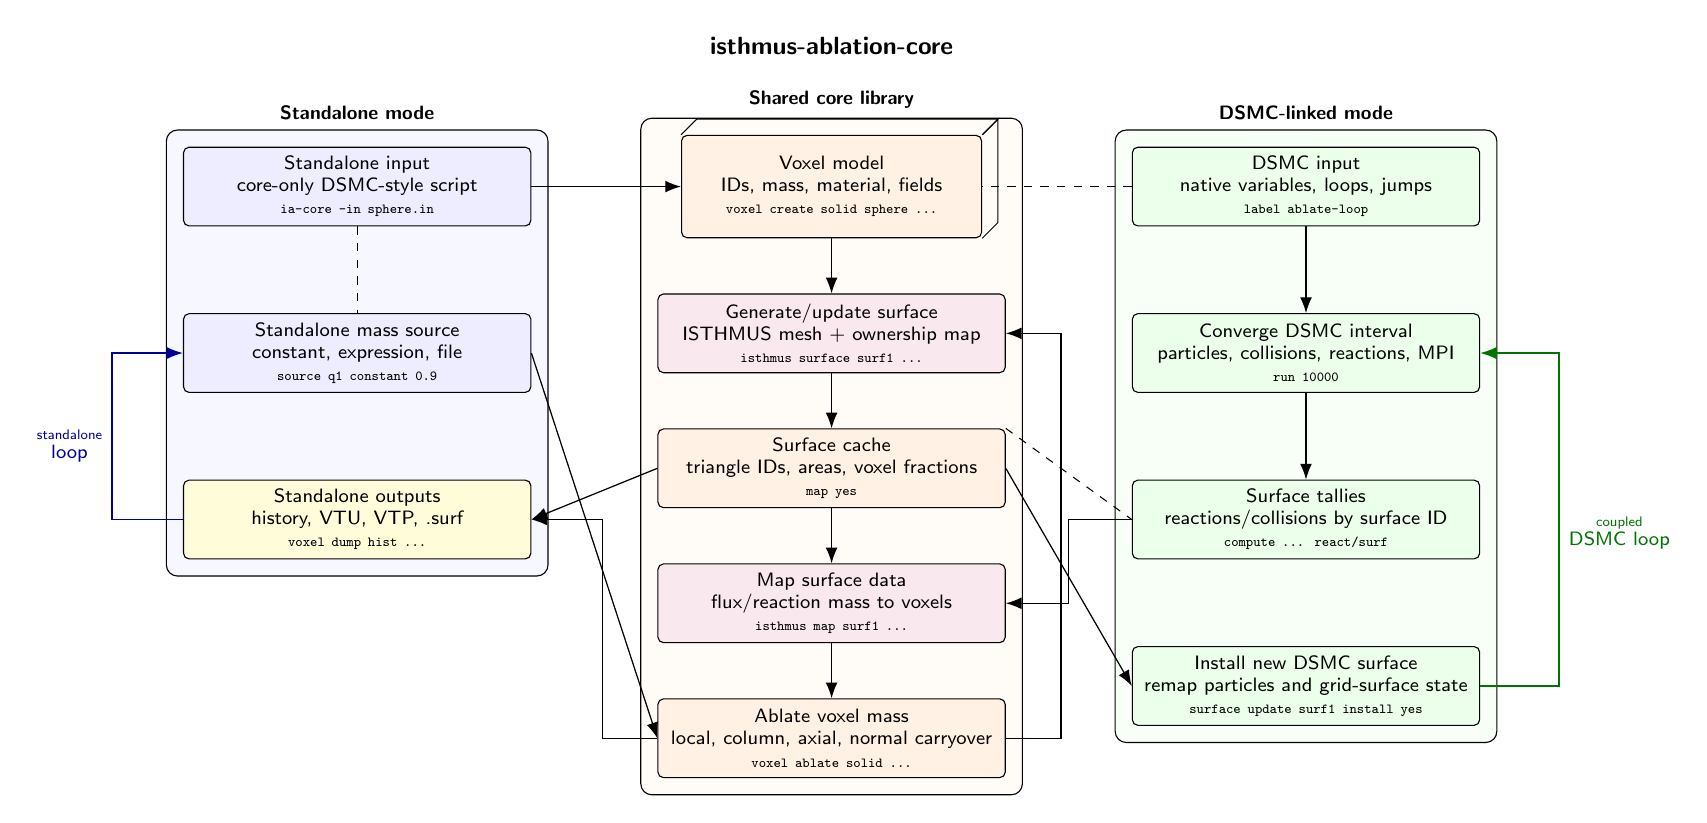
\begin{tikzpicture}[
  font=\sffamily\scriptsize,
  node distance=7mm and 10mm,
  box/.style={
    draw,
    rounded corners=2pt,
    align=center,
    text width=34mm,
    minimum height=10mm,
    inner sep=3pt
  },
  widebox/.style={
    box,
    text width=42mm
  },
  voxelbox/.style={
    box,
    text width=36mm,
    minimum height=13mm
  },
  group/.style={
    draw,
    rounded corners=4pt,
    inner sep=6pt
  },
  seqarrow/.style={
    -{Latex[length=2.0mm]},
    line width=0.45pt
  },
  looparrow/.style={
    -{Latex[length=2.1mm]},
    line width=0.55pt
  },
  connect/.style={
    dashed,
    line width=0.38pt
  },
  cmd/.style={
    font=\ttfamily\tiny
  }
]

\node[font=\sffamily\bfseries\small] (title) at (0,0) {isthmus-ablation-core};

% Shared core
\node[voxelbox, fill=orange!10, below=9mm of title] (voxels) {
  Voxel model\\
  IDs, mass, material, fields\\
  {\ttfamily\tiny voxel create solid sphere ...}
};
\draw[line width=0.38pt] (voxels.north east) -- ($(voxels.north east)+(2mm,2mm)$)
  -- ($(voxels.north west)+(2mm,2mm)$) -- (voxels.north west);
\draw[line width=0.38pt] (voxels.north east) -- ($(voxels.north east)+(2mm,2mm)$)
  -- ($(voxels.south east)+(2mm,2mm)$) -- (voxels.south east);

\node[widebox, fill=purple!9, below=of voxels] (isthmus) {
  Generate/update surface\\
  ISTHMUS mesh + ownership map\\
  {\ttfamily\tiny isthmus surface surf1 ...}
};

\node[widebox, fill=orange!10, below=of isthmus] (surface) {
  Surface cache\\
  triangle IDs, areas, voxel fractions\\
  {\ttfamily\tiny map yes}
};

\node[widebox, fill=purple!9, below=of surface] (map) {
  Map surface data\\
  flux/reaction mass to voxels\\
  {\ttfamily\tiny isthmus map surf1 ...}
};

\node[widebox, fill=orange!10, below=of map] (ablate) {
  Ablate voxel mass\\
  local, column, axial, normal carryover\\
  {\ttfamily\tiny voxel ablate solid ...}
};

% Standalone side
\node[widebox, fill=blue!7, left=19mm of voxels] (standalone_input) {
  Standalone input\\
  core-only DSMC-style script\\
  {\ttfamily\tiny ia-core -in sphere.in}
};

\node[widebox, fill=blue!7, below=11mm of standalone_input] (standalone_source) {
  Standalone mass source\\
  constant, expression, file\\
  {\ttfamily\tiny source q1 constant 0.9}
};

\node[widebox, fill=yellow!15, below=11mm of standalone_source] (standalone_output) {
  Standalone outputs\\
  history, VTU, VTP, .surf\\
  {\ttfamily\tiny voxel dump hist ...}
};

% DSMC side
\node[widebox, fill=green!8, right=19mm of voxels] (dsmc_input) {
  DSMC input\\
  native variables, loops, jumps\\
  {\ttfamily\tiny label ablate-loop}
};

\node[widebox, fill=green!8, below=11mm of dsmc_input] (dsmc_run) {
  Converge DSMC interval\\
  particles, collisions, reactions, MPI\\
  {\ttfamily\tiny run 10000}
};

\node[widebox, fill=green!8, below=11mm of dsmc_run] (tallies) {
  Surface tallies\\
  reactions/collisions by surface ID\\
  {\ttfamily\tiny compute ... react/surf}
};

\node[widebox, fill=green!8, below=11mm of tallies] (bridge) {
  Install new DSMC surface\\
  remap particles and grid-surface state\\
  {\ttfamily\tiny surface update surf1 install yes}
};

% Sequential standalone loop
\draw[seqarrow] (standalone_input) -- (voxels);
\draw[seqarrow] (voxels) -- (isthmus);
\draw[seqarrow] (standalone_source.east) -- (ablate.west);
\draw[seqarrow] (isthmus) -- (surface);
\draw[seqarrow] (surface) -- (map);
\draw[seqarrow] (map) -- (ablate);
\draw[seqarrow] (surface.west) -- (standalone_output.east);
\draw[seqarrow] (ablate.west) -- ++(-7mm,0) |- (standalone_output.east);
\draw[looparrow, blue!60!black] (standalone_output.west) -- ++(-9mm,0)
  |- (standalone_source.west)
  node[pos=0.22, left, align=center] {\tiny standalone\\[-1pt]loop};

% Sequential DSMC loop
\draw[seqarrow] (dsmc_input) -- (dsmc_run);
\draw[seqarrow] (dsmc_run) -- (tallies);
\draw[seqarrow] (tallies.west) -- ++(-8mm,0) |- (map.east);
\draw[seqarrow] (ablate.east) -- ++(7mm,0) |- (isthmus.east);
\draw[seqarrow] (surface.east) -- (bridge.west);
\draw[looparrow, green!45!black] (bridge.east) -- ++(10mm,0)
  |- (dsmc_run.east)
  node[pos=0.23, right, align=center] {\tiny coupled\\[-1pt]DSMC loop};

% Non-sequential relationships
\draw[connect] (surface.north east) -- (tallies.west);
\draw[connect] (standalone_input.south) -- (standalone_source.north);
\draw[connect] (dsmc_input.west) -- (voxels.east);

% Group boxes
\begin{scope}[on background layer]
  \node[group, fit=(standalone_input)(standalone_source)(standalone_output),
        fill=blue!3,
        label={[font=\sffamily\bfseries\scriptsize]above:Standalone mode}] {};

  \node[group, fit=(dsmc_input)(dsmc_run)(tallies)(bridge),
        fill=green!3,
        label={[font=\sffamily\bfseries\scriptsize]above:DSMC-linked mode}] {};

  \node[group, fit=(voxels)(ablate)(isthmus)(surface),
        fill=orange!3,
        label={[font=\sffamily\bfseries\scriptsize]above:Shared core library}] {};
\end{scope}

\end{tikzpicture}
\end{document}
